\section{Аймаг сумдын мэдээлэл авдаг форм}

Уг формыг шаардлагын дагуу алхам алхмаар хөгжүүлснээр React-н анхан шатны туршлагатай болох зорилготой байсан ба цаашид ажилласан төсөл дээр хэрэглэж буй зарим сан болох Material-ui, react-select-н ажиллагааг ойлгох, тодорхой хэмжээнд практик мэдлэгийг цуглуулж чадсан. 

Сурах ур чадвар: 
\begin{itemize}
    \item Асуудлаа тодорхойлж бага багаар шийдвэрлэх чадварт суралцах
    \item Git ашиглах чадвараа нэмэгдүүлэх
    \item Нэг төсөл дээр өөр өөр технологи ашиглах
\end{itemize}

Формын шаардлага: 
\begin{itemize}
    \item Next.js ашигласан байна
    \item Functional component ашиглаж, тухайн component-н дотоод төлвийг ашиглах
    \item Эцэг сонголтыг өөрчлөхөд хүү сонголтуудын утга цэвэрлэгддэг байх
    \item useEffect hook ашиглах
    \item Дараагийн шатанд форм дээрээ Material-ui нэвтрүүлэх
    \item Дараагийн шатанд useReducer ашиглах
    \item Дараагийн шатанд react-select санг нэвтрүүлэх
\end{itemize}

\subsection{useEffect болон useState ашиглан формын мэдээллийг шаардлагын дагуу авах}

Эхний ээлжинд ямар нэгэн загваргүй зөвхөн формын зөв ажиллагаа буюу логик үйлдлүүд дээр анхаарах хэрэгтэй байсан ба хамгийн түрүүнд хийх шаардлагатай зүйл нь аймаг сумдын датаг next.js дээрээ үүсгэсэн api-аасаа авч дэлгэцэнд харуулах байсан юм. 

\begin{lstlisting}[language=Javascript, caption=Next.js дээр бичсэн серверээс датагаа татаж авах, frame=single]
const fetchData = (url) => {
  return axios
    .get(`http://localhost:3000/api/${url}`)
    .then((res) => {
      const results = res.data;
      return results;
    })
    .catch((err) => {
      console.error(err);
    });
};
\end{lstlisting}

Доор харагдаж буй хэсэгт компонентийн логик үйлдлүүд харагдаж байна. useForm() hook ашиглаж select-н утга өөрчлөгдсөн эсэхийг барьж авах, functional component ашиглан state дотор хэрэглэгчийн сонгосон аймаг, сум, хороог хадгална. 

\begin{lstlisting}[language=Javascript, caption=Component-н үндсэн логик үйлдлүүд, frame=single]
export default function Home() {
  const [values, handleChange] = useForm();
  const [data, setData] = useState({
    cities: [],
    districts: [],
    wards: [],
  });

  useEffect(() => {
    fetchData(`cities`)
      .then((res) => {
        setData({ ...data, cities: res });
      })
      .catch((err) => {
        console.error(err);
      });
  }, []);

  const register = (e) => {
    e.preventDefault();
    console.log(values);
  };

  const handleSelect = (id, type) => {
    if (type == "city") {
      fetchData(`cities/${id}`)
        .then((res) => {
          setData({ ...data, districts: res, wards: [] }); //set districts and clear wards data
        })
        .catch((err) => {
          console.error(err);
        });
    } else if (type == "district") {
      //get wards
      fetchData(`cities/${values.city}/${id}`)
        .then((res) => {
          setData({ ...data, wards: res });
        })
        .catch((err) => {
          console.error(err);
        });
    }
  };
  
  ...
\end{lstlisting}

State дотор хэрэглэгчийн сонгосон мэдээллийг зөвөөр хадгалах шаардлагатай байсан. Эхний байдлаар доор харагдаж байгаагаар хадгалсан ч үүссэн асуудлууд нь замбаараагүй, эцэг сонголтыг сонгоход хүү сонголтуудыг цэвэрлэхэд төвөгтэй байв.

\begin{lstlisting}[language=Javascript, caption=Дотоод төлвийн эхний хувилбар, frame=single]
	const [cities, setCities] = useState([]);
  const [districts, setDistricts] = useState([]);
  const [wards, setWards] = useState([]);
  const [selectedCity, setSelectedCity] = useState();
  const [selectedDistrict, setSelectedDistrict] = useState();
  const [selectedWard, setSelectedWard] = useState();
\end{lstlisting}

Иймд state-ээ дараах байдлаар хадгаллаа.

\begin{lstlisting}[language=Javascript, caption=Дотоод төлвийн сайжруулсан хувилбар, frame=single]
	const [data, setData] = useState({
    cities: [],
    districts: [],
    wards: [],
  });
\end{lstlisting}

Эхний шаардлагын дагуу формыг хэрэгжүүлсний дараах вэб дээр харагдах байдал

\begin{figure}
	\centering
	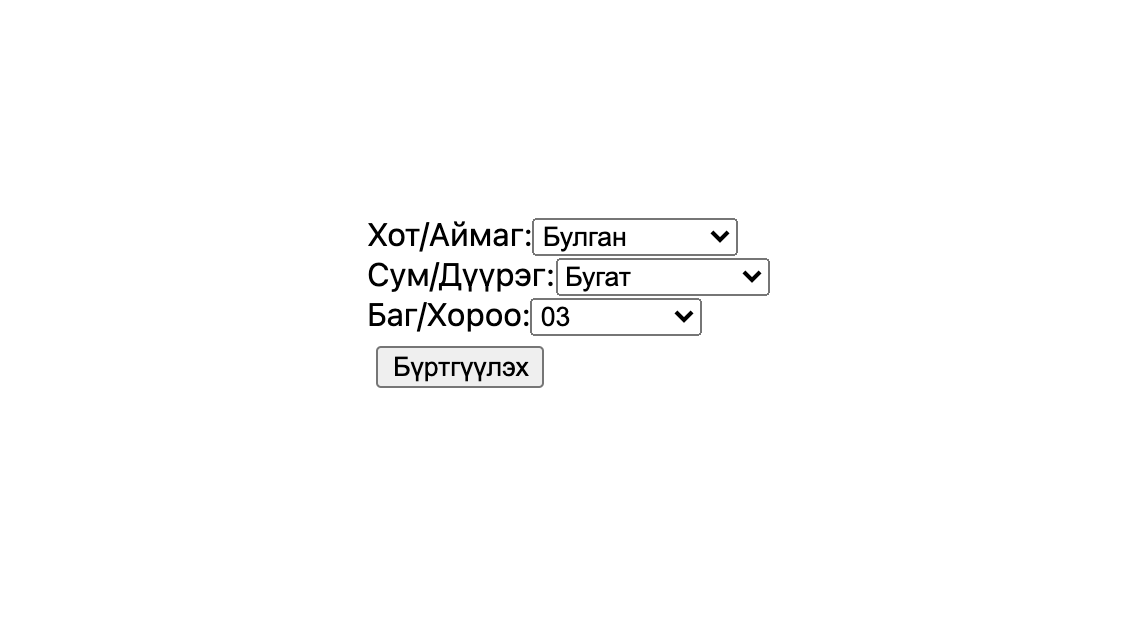
\includegraphics[width=15cm]{images/form-v1.png}
	\caption{Формын эхний хувилбар}
	\label{fig:my_label}
\end{figure}

\pagebreak
\subsection{useState-н оронд useReducer hook ашиглах}

useReducer нь useState hook-н өөр нэг хувилбар бөгөөд өөр дээрээ state болон action гэсэн параметрүүдийг хүлээн авдаг. State нь өгөгдөл хадгалах бол action нь тухайн state дээр ямар үйлдлүүдийг хийх шаардлагатайг хүлээж авдаг. 

Хамгийн түрүүнд Action-ынхаа төрлүүдийг зарлана.

\begin{lstlisting}[language=Javascript, caption=Хийх үйлдлүүдийн төрлийг зарлах, frame=single]
	const SET_CITY = "city";
	const SET_DISTRICT = "district";
	const SET_WARD = "ward";
\end{lstlisting}

Үүний дараа хийх үйлдлүүдээ switch case дотор тодорхойлно. Switch case ашигласнаар олон дахин функц зарлах шаардлагагүйгээр Action-н төрлөөс хамаарч тухайн үйлдлийг ажиллуулна. 

\begin{lstlisting}[language=Javascript, caption=Хийх үйлдлүүдийг тодорхойлох, frame=single]
	const reducer = (state, action) => {
  switch (action.type) {
    case SET_CITY:
      return {
        city: action.index,
        district: null,
        ward: null,
      };
    case SET_DISTRICT:
      return {
        ...state,
        district: action.index,
        ward: null,
      };
    case SET_WARD:
      return {
        ...state,
        ward: action.index,
      };
    default:
      return state;
  }
};
\end{lstlisting}

useReducer ашигласнаар өгсөн шаардлагуудын нэг болох эцэг сонголтыг солиход хүү сонголтууд хоосрох ёстой гэснийг маш хялбар байдлаар шийдэх боломжтой болов. Ердөө тухайн сонголтын доор байгаа state-үүдийн утгыг анхны утгаар солисон.

\begin{lstlisting}[language=Javascript, caption=Хүү сонголтуудыг цэвэрлэх, frame=single]
	...
    case SET_DISTRICT:
      return {
        ...state,
        district: action.index,
        ward: null,
      };
  ...
\end{lstlisting}

Одоо форм дээрээ React-Select санг ашиглаж компонент доторх кодоо бичих шаардлагатай. Энэ хэсэг нь DOM дээр рендерлэгдэнэ. 

\begin{lstlisting}[language=Javascript, caption=React-Select ашигласан байдал, frame=single]
	...  
	<form className={styles.grid} onSubmit={register}>
		<label>
			<p>Country:</p>
			<Select
				value={address.map((i, index) => ({ ...i, index }))[state.city]}
				onChange={(e) => handleChange(e.index, SET_CITY)}
				options={address.map((i, index) => ({ ...i, index }))}
				getOptionLabel={(option) => option.name}
				getOptionValue={(option) => option.index}
				placeholder="Choose country"
			/>
		</label>
  ...
\end{lstlisting}
\pagebreak

React-Select болон Material-UI ашигласны дараа формын маань харагдах байдал. Удирдагчийн өгсөн шаардлагуудын дагуу амжилттай хөгжүүлж дууслаа.
\begin{figure}
	\centering
	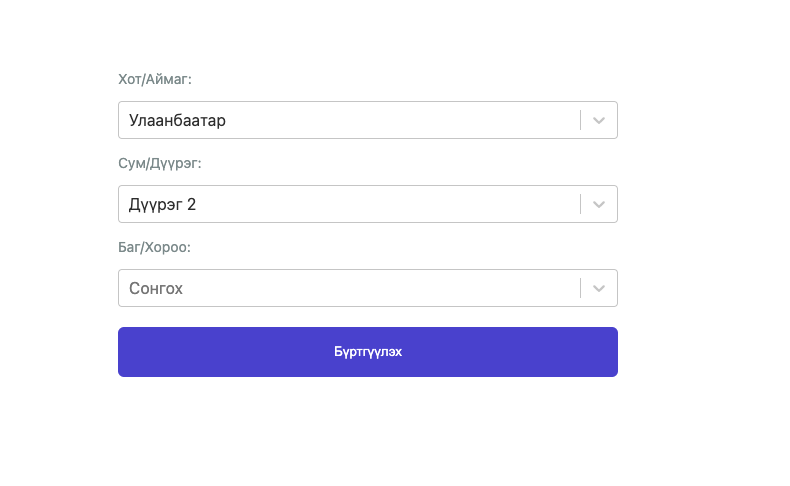
\includegraphics[width=15cm]{images/form.png}
	\caption{Формын эцсийн байдлаар харагдаж буй байдал}
	\label{fig:my_label}
\end{figure}
\pagebreak

\section{Toast компонент}

Уг компонентийн гол үүрэг нь Мерчант төсөл дээр ашиглаж буй бүх хүсэлтүүдийн хариуг хэрэглэгч дээр харуулах үүрэгтэй. Мөн хөгжүүлж дууссаны дараа хэрэглэгчийн интерфэйсийн автоматжуулсан тест хийж байж production дээр орох боломжтой.

Сурах ур чадвар: 
\begin{itemize}
    \item State management-н гол ойлголт болох Context-н талаар мэдлэгтэй болно
    \item Өөрийн шаардлагад нийцсэн custom hook бичиж сурах
    \item Хэрхэн бичсэн компонент дээрээ UI автоматжуулсан тест бичих мэдлэг
\end{itemize}

Формын шаардлага: 
\begin{itemize}
    \item Material-UI-н Snackbar ашиглах
    \item Олон Toast зэрэг гаргадаг байх
    \item Toast нь үүсгэх, цэвэрлэх, устгах үйлдлүүдтэй байх
    \item Toast-н цаг дуусахад автоматаар цэвэрлэдэг байх
    \item UI автоматжуулсан тестийг давсан байх
\end{itemize}

\subsection{Context үүсгэх}

React-н өгөгдлийн урсгал нэг чиглэлд буюу зөвхөн эцгээс хүү компонент рүү утга дамжуулах чадвартай байдаг. Иймд нэг state-ээ нэгэндээ хамааралгүй олон өөр газарт ашиглагдаж байгаа компонентод ашиглахын тулд маш замбаараагүй дамжуулалт хийх шаардлага гардаг. Харин үүний нэг шийдэл нь Context гэх ойлголт бөгөөд бусад програмчлалын хэл дээр байдаг Global хувьсагч шиг ашиглах боломжтой. 

Хамгийн эхлээд context-оо үүсгэж, түүний хийх үйлдлүүдийг зарлаж өгөх хэрэгтэй. Өмнөх хэрэгжүүлэлт дээр ашигласан useReducer-н мэдлэг хэрэг болов.

\begin{lstlisting}[language=Javascript, caption=Context үүсгэх, frame=single]
	...  
	export const ACTION_TOAST = "TOAST";
	export const ACTION_RESET = "RESET";
	export const ACTION_CLEAR = "CLEAR";

	export const INITIAL_STATE: { toasts: ToastType[] } = {
		toasts: [],
	};

	type Actions =
		| (ActionType<typeof ACTION_TOAST> & { toast: ToastType })
		| ActionType<typeof ACTION_RESET>
		| (ActionType<typeof ACTION_CLEAR> & { id: string });

	export const ToastContext = createContext(null);
	ToastContext.displayName = "ToastContext";
	export const ToastControlContext = createContext(null);
	ToastControlContext.displayName = "ToastControlContext";
  ...
\end{lstlisting}

Toast-н анхны утгыг зарласан байдал 

\begin{lstlisting}[language=Javascript, caption=Toast context-н анхны утгыг зарласан байдал, frame=single]
	...  
	export const INITIAL_STATE: { toasts: ToastType[] } = {
		toasts: [],
	};
  ...
\end{lstlisting}

Мөн манайх төсөл дээрээ Typescript ашигладаг тул мэдээж Toast-н интерфэйсийг зааж өгөх хэрэгтэй. Ингэснээр Toast ашиглаж буй хөгжүүлэгч тухайн компонент ямар төрөлтэй ямар props-уудыг хүлээн авах шаардлагатайг хялбараар харах боломжтой. Мөн хөгжүүлэлтийн явцад гарах алдаа багасна.

\begin{lstlisting}[language=Javascript, caption=Toast-н интерфэйс тодорхойлох, frame=single]
	...  
	export interface ToastType {
		id?: string;
		message: string;
		type: "success" | "info" | "warning" | "error";
		duration?: number;
	}
  ...
\end{lstlisting}

Одоо шаардлагын дагуу Toast үүсгэх, цэвэрлэх, устгах үйлдэл хийх функцын кодыг бичсэн

\begin{lstlisting}[language=Javascript, caption=Toast үүсгэх функц, frame=single]
	...  
	function toast(state: typeof INITIAL_STATE, toast: ToastType): typeof state {
		return {
			...state,
			toasts: [...state.toasts, toast],
		};
	}
  ...
\end{lstlisting}

\begin{lstlisting}[language=Javascript, caption=Toast-г context-оос цэвэрлэх, frame=single]
	...  
	function clear(state: typeof INITIAL_STATE, toastId: string): typeof state {
		return {
			...state,
			toasts: state.toasts.filter((toast) => toast.id !== toastId),
		};
	}
  ...
\end{lstlisting}

Олон Toast зэрэг гарах боломжтой тул үүсгэсэн Toast бүр дээрээ uniq ID үүсгэж, түүний дараа тухайн ID-аар нь хайж олон цэвэрлэх боломжтой болно. 

\begin{lstlisting}[language=Javascript, caption=Uniq ID гаргах, frame=single]
	...  
	function generateToastId() {
		return Math.random().toString(36).substr(2, 9);
	}
  ...
\end{lstlisting}

Тухайн үйлдлийг дуудахад дээр тодорхойлж өгсөн тус тусын үүрэгтэй функцууд ажиллана. Бүх Toast-г context дотроосоо устгахдаа case дээр анхны зарласан хоосон массивыг буцааж оноож байгаа. 

\begin{lstlisting}[language=Javascript, caption=useReducer дээр ажиллах үйлдлүүдийг заах, frame=single]
	...  
	function reducer(state = INITIAL_STATE, action: Actions): typeof state {
		switch (action.type) {
			case ACTION_TOAST:
				return toast(state, action.toast);
			case ACTION_RESET:
				return INITIAL_STATE;
			case ACTION_CLEAR:
				return clear(state, action.id);
			default:
				return state;
		}
	}
  ...
\end{lstlisting}

\subsection{Custom Hook бичих}

Hook бичиж өгснөөр Toast-г бүрэн ашиглах нөхцөл нь бүрдэнэ. useToast() болон useToastControl() гэсэн хоёр төрлийн hook бичиж өгсөн. 

Тухайн context-г төсөл дотор буюу index.jsx файлд wrap хийж өгөөгүй нөхцөлд console дээр ашиглах боломжгүй гэсэн алдааг гаргаж өгөх шаардлагатай.

\begin{lstlisting}[language=Javascript, caption=Context-г буруу ашигласан үед алдаа гаргах, frame=single]
	...  
	export function useToastControl() {
		const dispatch = useContext(ToastControlContext);
		if (!dispatch) throw new TypeError("Please use within ToastProvider");

		const reset = useCallback(() => dispatch({ type: ACTION_RESET }), [dispatch]);
  ...
\end{lstlisting}

Toast-г шинээр үүсгэх шаардлагатай үед уг код ажиллана. Хэрэв Toast-оо үүсгэхдээ дэлгэцэнд харагдах цагийг зааж өгөөгүй бол автоматаар 4000 ms-н дараа тухайн Toast санах ой болон хэрэглэгч дээр харагдах хэсгээс цэвэрлэгдэнэ.

\begin{lstlisting}[language=Javascript, caption=Toast үүсгэх үүрэгтэй hook, frame=single]
	...  
	const toast = useCallback(
    (toast: ToastType) => {
      const toastId = generateToastId();

      dispatch({ toast: { ...toast, id: toastId }, type: ACTION_TOAST });

      setTimeout(() => {
        dispatch({ id: toastId, type: ACTION_CLEAR });
      }, toast.duration || 4000);
    },
    [dispatch]
  );
  ...
\end{lstlisting}

Үүний дараа Toast компонентийнхоо интерфэйсийг Material-UI сан ашиглаж шийдэв.


\begin{lstlisting}[language=Javascript, caption=Material-UI ашиглаж интерфэйсийг үүсгэх, frame=single]
	...  
	return (
		<Snackbar
			anchorOrigin={{ horizontal: "center", vertical: "bottom" }}
			open={open}
			autoHideDuration={duration}
			onClose={onClose}
			action={action}
		>
			<Alert onClose={onClose} severity={type} sx={{ width: "100%" }}>
				{message}
			</Alert>
		</Snackbar>
	);
  ...
\end{lstlisting}

Hook бичихгүйгээр шийдэх нь Toast-г ашиглахын тулд бүтэн компонент код бичих асуудалтай байсан ба custom hook-р шийдсэнээр хөгжүүлэгч ердөө ганц функцийг л дуудаж ажиллуулахад хангалттай. Ингэснээр хөгжүүлэлтийн хурданд ч эерэгээр нөлөөлнө. 

\begin{lstlisting}[language=Javascript, caption=Toast-г дуудаж ашиглаж буй байдал, frame=single]
	...  
	.then(
        (res) =>
          res.data &&
          toast({
            message: "Created product",
            type: "success",
          })
      )
  ...
\end{lstlisting}
\pagebreak

\section{UI автоматжуулсан тест}

Бичсэн компонентдоо тест код бичсэнээр ажиллагааг нь баталгаажуулах, алдааг илрүүлэх, хүнээр тест хийлгүүлэх шаардлагагүй болдог. Тестээ бичихдээ React багийн гишүүн Kent C. Dodds-н Jest сан дээр нэмэлт хөгжүүлэлт хийж гаргасан React Testing Library ашиглав.

Хуурамч цаг ашиглаж, тест хийх stage-н хурдыг нэмэгдүүлнэ. Ингэснээр заавал Toast дээр тавигдсан 4 секундыг хүлээх хэрэггүй.

\begin{lstlisting}[language=Javascript, caption=FakeTimer ашиглах, frame=single]
	...  
	jest.useFakeTimers();
  ...
\end{lstlisting}

Хамгийн эхэнд хийгдэх тест бол DOM дээр зурагдаж байгаа эсэх, явуулсан string-г хэвлэж байгаа эсэх болон "ХААХ" товчлуур дээр дарагдахад цэвэрлэгдэж байгаа эсэхийг шалгах юм.

\begin{lstlisting}[language=Javascript, caption=Toast компонентийг DOM дээр зурна, frame=single]
	...  
	const message = "Hello, it's toast";
  render(<Toast message={message} type="success" />);
  ...
\end{lstlisting}

\begin{lstlisting}[language=Javascript, caption=DOM дээр зурагдсан эсэхийг шалгана, frame=single]
	...  
	expect(screen.getByText(message)).toBeInTheDocument();
  ...
\end{lstlisting}

\begin{lstlisting}[language=Javascript, caption=Хаах товчлуур дээр дарахад устсан эсэхийг шалгах, frame=single]
	...  
	userEvent.click(
    screen.getByRole("button", {
      name: /close/i,
    })
  );

  await waitForElementToBeRemoved(() => screen.getByText(message));

  expect(screen.queryByText(message)).not.toBeInTheDocument();
  ...
\end{lstlisting}

Үүний дараачаар компонентийг хоёр удаа дуудаж ажиллуулаад интерфэйс дээр харагдах нийт хугацааг өөр өөрөөр зааж өгнө. Хөгжүүлэгч дурын хугацаа зааж өгсөн үед уг хугацааны үед ажиллаж байгаа эсэхийг шалгана.

\begin{lstlisting}[language=Javascript, caption=Олон Toast зэрэг гаргаж дурын хугацааг зааж өгөх, frame=single]
	...  
	test("duration", async () => {
    const cssAnimation = 300;
    const toasts = [
      {
        duration: 4000,
        message: "Toast 1",
      },
      {
        duration: 5000,
        message: "Toast 2",
      },
  ];

  toasts.forEach((toast) =>
      render(
        <Toast
          message={toast.message}
          type="success"
          duration={toast.duration}
        />
      )
  );
  ...
\end{lstlisting}

\begin{lstlisting}[language=Javascript, caption=Зааж өгсөн хугацааны дараа цэвэрлэгдэж байгаа эсэхийг шалгах, frame=single]
	...  
	expect(screen.getByText("Toast 1")).toBeInTheDocument();
    await waitForElementToBeRemoved(() => screen.getByText("Toast 1"), {
      timeout: toasts[0].duration + cssAnimation,
    });
  expect(screen.queryByText("Toast 1")).not.toBeInTheDocument();
  ...
\end{lstlisting}

Хамгийн сүүлд нь миний бичсэн Toast дөрвөн өөр төрлийг хүлээж аваад тухайн төрлөөс нь хамаарч өөр загвартай харуулдаг тул уг төрлийн дагуу зурагдаж байгаа эсэхийг шалгах юм. 

Toast-н хүлээж авах type-н жагсаалт:
\begin{itemize}
	\item success
	\item info
	\item warning
	\item error
\end{itemize}

\begin{lstlisting}[language=Javascript, caption=Өгсөн type-н дагуу зурагдаж байгаа эсэхийг шалгах, frame=single]
	...  
	test("check type", () => {
    const types = [
      {
        class: "filledSuccess",
        message: "Success toast",
        type: "success",
      },
      { class: "filledError", message: "Error toast", type: "error" },
      { class: "filledInfo", message: "Info toast", type: "info" },
      {
        class: "filledWarning",
        message: "Warning toast",
        type: "warning",
      },
    ];

  types.forEach((opt) => {
    const { container } = render(
      <Toast
        message={opt.message}
        type={opt.type as "success" | "info" | "warning" | "error"}
      />
    );
    const alert = container.firstChild;

    expect(alert.firstChild).toHaveClass(`MuiAlert-${opt.class}`);
    cleanup();
    });
  });
  ...
\end{lstlisting}



